\documentclass[a4paper, 11pt]{exam}
\usepackage{titling}
\newcommand{\subtitle}[1]{%
  \posttitle{%
    \par\end{center}
    \begin{center}\large#1\end{center}
    }%
}

\usepackage{url}
\usepackage{amsmath,amsthm,enumitem,amssymb}
\usepackage{algorithm,algorithmic,amsmath}
\usepackage{graphicx}
\usepackage{hyperref}
\renewcommand{\labelenumii}{\roman{enumii}}
\usepackage{courier}
\usepackage{epsfig}

\title{Homework Assignment 4}
\subtitle{CS/ECE 6810: Computer Architecture \\
Nov 28, 2018\\
Jake Pitkin, u0891770}

\author{ \\
\textbf{Memory Systems}}
\date{Due Date: December 11, 2018.\\
(120 points)}

\begin{document}
\maketitle

\begin{enumerate}

\item \textbf {Virtually Indexed Cache.}
Referring to the lecture slide on virtual address translation and TLB, explain the
challenges if the number of bits in the page offset does not equal the number of
bits in the sum of ``Index'' and ``Byte'' (Please see \url{http://www.cs.utah.edu/~bojnordi/classes/6810/f18/slides/18-tlb.pdf}). 
You are asked to identify the issues and their corresponding solutions from the literature.
\textbf{(20 points)}

Let x be the number of page offset bits and y be the number of bits in the sum of "Index" and "Byte". We will consider 3 cases: \\

\textbf{Case x = y:} In this case they are equal, there is no challenge and we can index into the cache in parallel with page number translation by the TLB. This is a side effect of the page offset bits being identical in both the virtual and physical addresses so waiting for the TLB to execute won't change the bits used for "Index" and "Byte". \\

\textbf{Case x $>$ y:} Here we have more page offset bits than required for "Index" and "Byte". We can just use a subset of the page offset bits for "Index" and "Byte" and this is fine for the same reasons as in case 1. \\

\textbf{Case x $<$ y:} When there are less page offset bits than required for "Index" and "Byte" an issue arises. As discussed in the lecture, in this case part of the "Index" bits will come from the virtual address. This means the index into cache will be dependent on the virtual address. Two different virtual addresses could be mapped to a single physical address. As such, it's possible for a given physical word to be put into the cache in more than one location. \\

From the wikipedia on CPU caches, this is called aliasing. This is an issue as we now have cache coherence problems inside a single cache. Processors are designed to satisfy cache coherence under the assumption a given cache only contains a physical word once. There is also the issue of contiguous pages in virtual memory not always being contiguous in physical memory. Using the virtual address for caching could lead to poor performance as we overwrite contiguous pages in physical memory.\\

To solve this issue we must guarantee any given physical word doesn't exist in a cache in more than one location. But we still want to use the virtual address for some of the "Index" bits as it allows us to run the two streams of execution as described in the lecture. As hinted in lecture the solution is cache coloring.\\

From the wikipedia on cache coloring, it is the process of attempting to allocate free pages that are contiguous from the CPU cache's point of view. That is, normally a physically index CPU aims to place contiguous pages in physical memory in different positions in the cache. But with page coloring: \textit{Physical memory pages are "colored" so that pages with different "colors" have different positions in CPU cache memory. When allocating sequential pages in virtual memory for processes, the kernel collects pages with different "colors" and maps them to the virtual memory. In this way, sequential pages in virtual memory do not contend for the same cache line} (from the wikipedia on cache coloring). \\

This solves our performance problem as sequential pages in virtual memory do not content for the same cache line. When using some of the virtual address bits for "Index" we use the lower bits. As such, contiguous pages in virtual memory will be assigned different positions in the cache. Additionally this solves the problem of aliasing. If two virtual addresses map to the same physical address, they will be assigned to the same line in the cache (as the physical address with have a given color) and we won't have duplicate entries and cache coherence problems.

\textbf{References:}

Lecture 18 video: https://web.microsoftstream.com/ \\ video/8d07bb10-4791-4c46-bab8-1b2e2a7e1a09 \\

Lecture 18 slides: http://www.cs.utah.edu/~bojnordi/classes/6810/f18/slides/18-tlb.pdf \\

Wikipedia on caches: https://en.wikipedia.org/wiki/CPU\_cache \\

Wikipedia on cache coloring: https://en.wikipedia.org/wiki/Cache\_coloring

\item \textbf {Virtual Memory and TLB.}
Consider an operating system (OS) using 1KB pages for mapping virtual to physical addresses.
Initially, the TLB is empty and all of the required pages for the user application as well as the page table are stored in the main memory.
(There is no need to transfer data between main memory and the storage unit.)
Every access to the TLB and main memory takes respectively 1 and 200 processor cycles.
The TLB can store up 16 entries.

\begin{enumerate}
	\item Assuming that the main memory size is 1MB and the page table has 2048 entries, show the number of required bits for the physical and virtual address fields. \textbf{(5 points)}
	
	1KB pages = $2^{10}$ = 10 offset bits to index \\
	2048 page table entries = $2^{11}$ =  11 bits to address \\
	1MB main memory with 1KB pages = $2^{20} / 2^{10}$ = 10 bits to address
	
	\fbox{\parbox{\linewidth}{
	Virtual address = Virtual Page No + offset = 11 + 10 = 21 bits \\
	Physical address = Page frame No + offset = 10 + 10 = 20 bits}}
	\item Assume that the user application only generates five memory requests to the virtual addresses \texttt{0000}, \texttt{0004}, \texttt{0008}, \texttt{0800}, and \texttt{0804} (all in hexadecimal);
	the first request is ready at time 0; and
	the processor generates every next request immediately after serving the current one.
	Please find the execution time with and without using TLB in the proposed system and compute the attainable speedup due to using TLB.
	\textbf{(15 points)}
	
	\textbf{Assumptions:} There is no mention of caching the words once they have been accessed. I will assume that once the virtual address has been translated to a physical address we will always have to access memory to get the data (as there is no caching). I'll also assume searching the page table takes negligible time as it's not mentioned in the problem. \\
	
	\textbf{Without a TLB:} every access will have to read the page table in main memory and the data in main memory as there is no caching: \\
	
	\begin{center}
	\begin{tabular}{ |c|c|c|c| } 
		\hline
		\textbf{Virtual Address}& \textbf{Virtual Page No} & \textbf{Offset} & \textbf{Access Cycles} \\ 
		\hline
		0000 & 0 & 0 & 400\\ \hline
		0004 & 0 & 8 & 400 \\ \hline
		0008 & 0 & 16 & 400 \\ \hline
		0800 & 2 & 0 & 400\\ \hline
		0804 & 2& 8 & 400 \\ \hline
	\end{tabular}
	\end{center}
	
	\fbox{2,000 cycles with no TLB}

	\textbf{With a TLB:} every access will still have to read main memory for the data as there is no caching, but we can cache address translations in the TLB:
	
	\begin{center}
	\begin{tabular}{ |c|c|c|c| } 
		\hline
		\textbf{Virtual Address}& \textbf{Virtual Page No} & \textbf{Offset} & \textbf{Access Cycles} \\ 
		\hline
		0000 & 0 & 0 & 400\\ \hline
		0004 & 0 & 8 & 201 \\ \hline
		0008 & 0 & 16 & 201 \\ \hline
		0800 & 2 & 0 & 400\\ \hline
		0804 & 2& 8 & 201 \\ \hline
	\end{tabular}
	\end{center}
	
	\fbox{1,403 cycles with a TLB}
	
	\textbf{Speedup:} to calculate speedup we compare the ratio of access cycles for not using a TLB and using a TLB:
	
	\fbox{old time / new time = 2,000 / 1,403 = 1.4255 or a 42.55\% speedup}
\end{enumerate}






\item \textbf {DRAM Address Mapping.}
Consider a simple in-order DRAM command scheduler.
Initially, all DRAM banks are precharged and the scheduling queue contains seven read requests to the following physical addresses: 
\texttt{00040108},
\texttt{01040101},
\texttt{FF042864},
\texttt{A5181234},
\texttt{A5184321},
\texttt{00161804}, and
\texttt{01040104}
(all in hexadecimal).
Using the following address mapping scheme, show all the required commands issued by the controller to serve the memory requests.
\textbf{(20 points)}

\begin{center}
	\begin{tabular}{|c|c|c|c|c|}
		\hline
		row (10)&bank (4)&rank (2)&channel (0)&column (16) \\
		\hline
	\end{tabular}
\end{center}

First I will calculate the row, bank, rank, and column from each physical address:


\begin{center}
	\begin{tabular}{ |c|c|c|c|c| } 
		\hline
		\textbf{Physical Address} & \textbf{row} & \textbf{bank} & \textbf{rank} & \textbf{column}\\ 
		\hline
		\texttt{00040108}  & 0 & 1 & 0 & 264 \\ \hline
		\texttt{01040101}  & 4 & 1 & 0 & 257\\ \hline
		\texttt{FF042864}  & 1020 & 1 & 0 & 10340\\ \hline
		\texttt{A5181234}  & 660 & 6 & 0 & 4660 \\ \hline
		\texttt{A5184321}  & 660 & 6 & 0 & 17185 \\ \hline
		\texttt{00161804}  & 0 & 5 & 2 & 6148 \\ \hline
		\texttt{01040104}  & 0 & 1 & 0 & 260\\ \hline
	\end{tabular}
\end{center}

\fbox{\parbox{\linewidth}{
Physical addresses are written in hex where the arguments for commands are in decimal. I am using the command representation presented in lecture 22 (RD commands).

\begin{center}
	\begin{tabular}{ |c|c| } 
		\hline
		\textbf{Physical Address}& \textbf{Commands}\\ 
		\hline
		\texttt{00040108} & ACT(0), RD(264)\\ \hline
		\texttt{01040101} & PRE, ACT(4), RD(257)\\ \hline
		\texttt{FF042864} & PRE, ACT(1020), RD(10340)\\ \hline
		\texttt{A5181234} & ACT(660), RD(4660)\\ \hline
		\texttt{A5184321} & RD(17185)\\ \hline
		\texttt{00161804} & ACT(0), RD(6148)\\ \hline
		\texttt{01040104} & PRE, ACT(0), RD(260)\\ \hline
	\end{tabular}
\end{center}

\textbf{Explanations:}\\

\textit{Access 00040108:} Bank 1 is already precharged so first we must activate row 0 and then read column 264. \\

\textit{Access 01040101:} The row buffer in bank 1 is not empty but this access is a miss. So we must prepare the row buffer with a precharage. Followed by activating row 4, and reading column 257 from the row buffer. \\

\textit{Access FF042864:} The row buffer in bank 1 is not empty but this access is a miss. So we must prepare the row buffer with a precharage. Followed by activating row 1020, and reading column 10340 from the row buffer. \\

\textit{Access A5181234:} Bank 6 is already precharged and the row buffer is empty so we activate row 660, and read column 4660 from the row buffer. \\

\textit{Access A5184321:} The bank 6 row buffer already contains row 660 so we just need to read column 17185 from the row buffer. \\

\textit{Access 00161804:} Bank 5 is already precharged and the row buffer is empty so we activate row 0, and read column 6148 from the row buffer. \\

\textit{Access 01040104:} The row buffer in bank 1 is not empty but this access is a miss. So we must prepare the row buffer with a precharage. Followed by activating row 4, and reading column 260 from the row buffer.
}}

\item \textbf{DRAM Row (Page) Management.}
A computer system includes DRAM and CPU.
The DRAM subsystem comprises a single channel/rank/bank.
CPU generates a sequence of memory requests to rows \texttt{X} and \texttt{Y}.
Table below shows the accessed rows by the memory requests and their arrival times at the DRAM controller.
Assume that the DRAM bank is precharged initially; the DRAM scheduling queue has infinite size; and the memory interface must enforce the following timing constraints (all in $ns$):
tCAS = 3, tRAS = 20, tRP = 20, tRCD = 10, and tBURST = 4. 

\begin{center}
	\begin{tabular}{|c|c|}
		\hline
		\textbf{Accessed Row} & \textbf{Arrival time ($ns$)} \\
		\hline
		\texttt{X}  & 10 \\
		\hline
		\texttt{X}  & 70 \\
		\hline
		\texttt{Y}  & 80 \\
		\hline
		\texttt{X}  & 85 \\
		\hline
		\texttt{Y}  & 110 \\
		\hline
		\texttt{X} & 210 \\
		\hline
	\end{tabular}
\end{center}

The goal is to evaluate two row management policies, namely \textit{open-page} and \textit{closed-page}.
Show all the necessary transactions on the command, address, and data buses for each policies.
Discuss which policy performs better for the given example.
(Note: you are allowed to reorder requests already waiting in the memory controller.)
\textbf{(20 points)}
\begin{figure}[h!]
	\begin{center}
		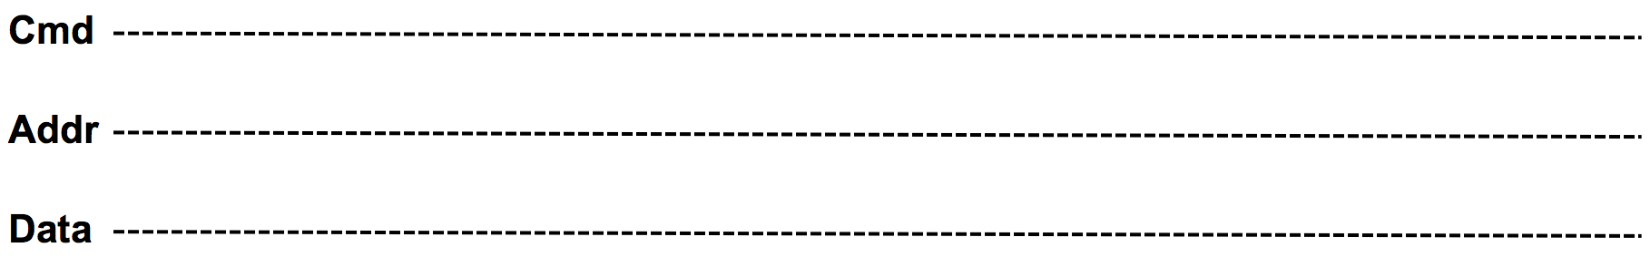
\epsfig{file=timing.pdf, width = \columnwidth}
	\end{center}
\end{figure}

First I will reorder the requests by swapping the 3rd and 4th request:

\begin{center}
	\begin{tabular}{|c|c|}
		\hline
		\textbf{Accessed Row} & \textbf{Arrival time ($ns$)} \\
		\hline
		\texttt{X}  & 10 \\
		\hline
		\texttt{X}  & 70 \\
		\hline
		\texttt{X}  & 85 \\
		\hline
		\texttt{Y}  & 80 \\
		\hline
		\texttt{Y}  & 110 \\
		\hline
		\texttt{X} & 210 \\
		\hline
	\end{tabular}
\end{center}

\textbf{Open-page policy:}

\begin{center}
	\begin{tabular}{|c|c|c|}
		\hline
		\textbf{Accessed Row} & \textbf{Arrival time ($ns$)} & \textbf{Complete time ($ns$)} \\
		\hline
		\texttt{X}  & 10 & 30\\
		\hline
		\texttt{X}  & 70 & \\
		\hline
		\texttt{X}  & 85 &\\
		\hline
		\texttt{Y}  & 80 &\\
		\hline
		\texttt{Y}  & 110 &\\
		\hline
		\texttt{X} & 210 &\\
		\hline
	\end{tabular}
\end{center}

\begin{center}
	\begin{tabular}{|c|c|c|c|c}}
		\hline
		\textbf{Cmd} & \textbf{Addr} & \textbf{Data} & \textbf{Time Start} & \textbf{Notes} \\
		\hline
		Act & X & - & 10 & 1\\ 
		\hline
		Rd & Col for request 1 & - & 20 &  1\\ 
		\hline
	\end{tabular}
\end{center}

\textbf{Closed-page policy:}

\item \textbf{Data TLB.}
Consider the following  pseudo code, in which \textbf{X} and \textbf{Y} are allocated as contiguous integer arrays in memory and are aligned to the 4KB boundaries.
Assume that \textbf{k} and \textbf{l} are allocated in the register file with no need for memory accesses.
We execute the code on a machine with virtual memory where the integer type (\textbf{int}) is 4 bytes wide.
Assume that the system include a direct-mapped D-TLB with 1024 entries for serving all data accesses only.
Initially, the D-TLB is empty.
Find the hit rate of the D-TLB when running the code.

\textbf{(20 points)}
\begin{algorithm}
	\textbf{\#define M 1024} \\
	\textbf{int X[M*M];} \\
	\textbf{int Y[M*M];} \\
	\textbf{int k, l;}
	\begin{algorithmic}	
		\FOR{$(k = 0; k < M; k++)$}
		\FOR{$(l = 0; l < M; l++)$}
		\STATE \texttt{Y[l*M+k] = X[k*M+l];}
		\ENDFOR
		\ENDFOR
	\end{algorithmic}
\end{algorithm}

\textbf{Virtual memory and TLB indexing} \\

We are using 4KB pages and 4 byte integers. The arrays are aligned to the 4KB boundary and each contain $2^{20}$ integers. Therefore each array is $4* 2^{20} = 2^{22}$ bytes long or 4,096KB. So we have 1,024 4KB pages for each array X and Y (in that order). \\

We will assume virtual memory only contains the 2,048 pages for X and Y and the page table has an entry for each. This requires 11 bits in the virtual address to index the page table. Our pages are 4KB so this requires 12 offset bits. We will assume the 11 virtual page number bits are the higher bits and the 12 offset bits are the lower bits. Giving a 23 bit virtual address.

\begin{center}
	\begin{tabular}{|c|c|}
		\hline
		Virtual Page Number 11 bits & Page Offset 12 bits\\
		\hline
	\end{tabular}
\end{center}

The direct mapped TLB contains 1,024 entries which requires 10 bits to index. I will assume we are using the lower 10 bits of the 11 virtual page number bits to index the TLB. The remaining bit will be a tag bit and we will still have 12 offset bits:

\begin{center}
	\begin{tabular}{|c|c|c|}
		\hline
		Tag 1 bit & TLB Index 10 bits & Page Offset 12 bits\\
		\hline
	\end{tabular}
\end{center}

An observation we can make is for some given index $i$, the address translation for $X[i]$ and $Y[i]$ will exist in the same row of the direct mapped TLB (with different tag bits). This is due to them being sequential in virtual memory and being conveniently sized and aligned. \\

\textbf{Access pattern of the code} \\

Now we can consider the access pattern of the virtual memory addresses. Given the arrangement of the code we will be accessing X and then Y (in that order) each iteration of the nested for-loops. \\

Given \texttt{X[k*M+l]} and the arrangement of the for-loops, each access to X will be sequential in memory (X[0], X[1], X[2], .... X[1,048,575]). \\

Given \texttt{Y[l*M+k]}, accesses to Y will not be sequential in memory (Y[0], Y[1,024], Y[2,048], ... Y[1,047,552], Y[1], Y[1,025], Y[2,049] ... Y[1,047,553], ...) but rather make 1,024 size hops until the end of the array is reached, increase by 1, and repeat 1,024 times. \\

\textbf{Hit rate of the D-TLB} \\

Let's just consider the first iteration of the inside for-loop. There will be 1,024 accesses to X that are sequential in memory X[0] - X[1023]. This will be a 4KB span of memory accesses as we are using 4 byte ints. So these accesses will only use one virtual page and one entry in the TLB (index 0 for the first iteration). \\

For the first iteration of the inside for-loop we will have memory accesses for Y as well. We will access Y[0], Y[1,024], Y[2,048], ..., Y[1,047,552]. These accesses will map to TLB indices 0, 1, ..., 1023 respectively.\\

The first iteration we will miss on X[0] (TLB index 0), miss on Y[0] (TLB index 0) and overwrite the TLB entry for X[0] (TLB index 0). The second iteration we will miss on X[1] (TLB index 0) and miss on Y[1,024] (TLB index 1). For the other 1,022 iterations we will hit on X[2]-X[1023] (TLB index 0) and Y will miss on every translation (TLB index 2 - 1023). Resulting in two misses for X and 1024 misses for Y. \\

Now the TLB contains translations for most of Y (TLB index 1 - 1023). Each iteration of the outside for-loop X will overwrite one of those entries (TLB entry $k$ from the outside for-loop), Y will overwrite TLB entry $k$ once and then X will restore it (similar to as described in the first iteration). Resulting in two misses for X and two misses for Y (TLB index $k$ from the previous and current iteration of the outside for-loop). \\

\fbox{\parbox{\linewidth}{First inside for-loop iteration X TLB hit rate: 1022/1024 \\
First inside for-loop iteration Y TLB hit rate: 0/1024 \\

Rest of inside for-loop iterations X TLB hit rate: 1022/1024 \\
Rest of inside for-loop iterations Y TLB hit rate: 1022/1024 \\

Address translations: 2 * 1024 * 1024 = 2,097,152 \\
Hits: 1 * (1022 + 0) + 1023 * (1022 + 1022) = 2,092,034 \\
Overall hit rate: $\frac{hits}{translations} = \frac{2,092,034}{2,097,152} = 0.9976 = 99.76\%$}}

\end{enumerate}
\end{document}
